\section{IBM Rational DOORS}
\label{chap:DOORS}

Das Anforderungsmanagement-Tool \ac{DOORS} ist ein plattformübergreifendes und unternehmensweites Tool und wird
zur Erfassung, Verknüpfung, Verfolgung, Analyse und Verwaltung von Anforderungen genutzt. \ac{DOORS} ist ein Akronym,
das für Dynamic Object-Oriented Requirements System steht. Alle Anforderungen und weitere Informationen werden in einer zentralen Datenbank
gespeichert. Innerhalb der Datenbank werden die Informationen in Modulen gespeichert. Diese Module können mithilfe von Ordnern und Projekten
organisiert werden. Ordner sind vergleichbar mit den Ordnern z.B. im Windows Explorer und können andere Ordner, Projekte oder Module
beinhalten. Ein Projekt hingegen ist ein spezieller Ordner, der alle Daten für ein entsprechendes Projekt beinhaltet. Sowohl für 
Ordner als auch für Projekte können die Zugriffsrechte individuell eingestellt werden \cite[vgl. S.173]{DOORS}. Dabei existieren die Optionen
read, modify, create, delete und administer (RMCDA). 

\subsection{Module}
Es existieren zwei verschiedene Arten von Modulen im Anforderungsmanagement-Tool \ac{DOORS}. Module, die die eigentlichen Anforderungen
beinhalten, werden Formal Module genannt. Abbildung \ref*{fig:Modul Doors} zeigt ein Beispiel für so ein Modul. Zu erkennen ist dort
ein geöffnetes Formal Module. Auf der linken Seite ist ein Explorer zu sehen, auf der rechten Seite die eigentlichen Inhalte des Moduls.
Durch den Explorer auf der linken Seite, der in einer Baumstruktur organisiert ist, wird es dem Benutzer ermöglicht leicht zu einer bestimmten
Stelle im Modul zu navigieren. Dabei können die einzelnen Sektionen auf- und zugeklappt werden \cite[vgl. S.176]{DOORS}. Die Daten auf der 
rechten Seite sind tabellarisch angeordnet. Die Spalten stellen dabei die einzelnen Attribute des Moduls dar, während die Zeilen die 
Objekte darstellen. 

Neben den Formal Modules existieren auch die Link Modules. In diesen werden Informationen über die Beziehungen zwischen einzelnen Objekten
gespeichert, was die Verfolgbarkeit von Anforderungen gewährleistet.

\begin{figure}[h]
    \centering
    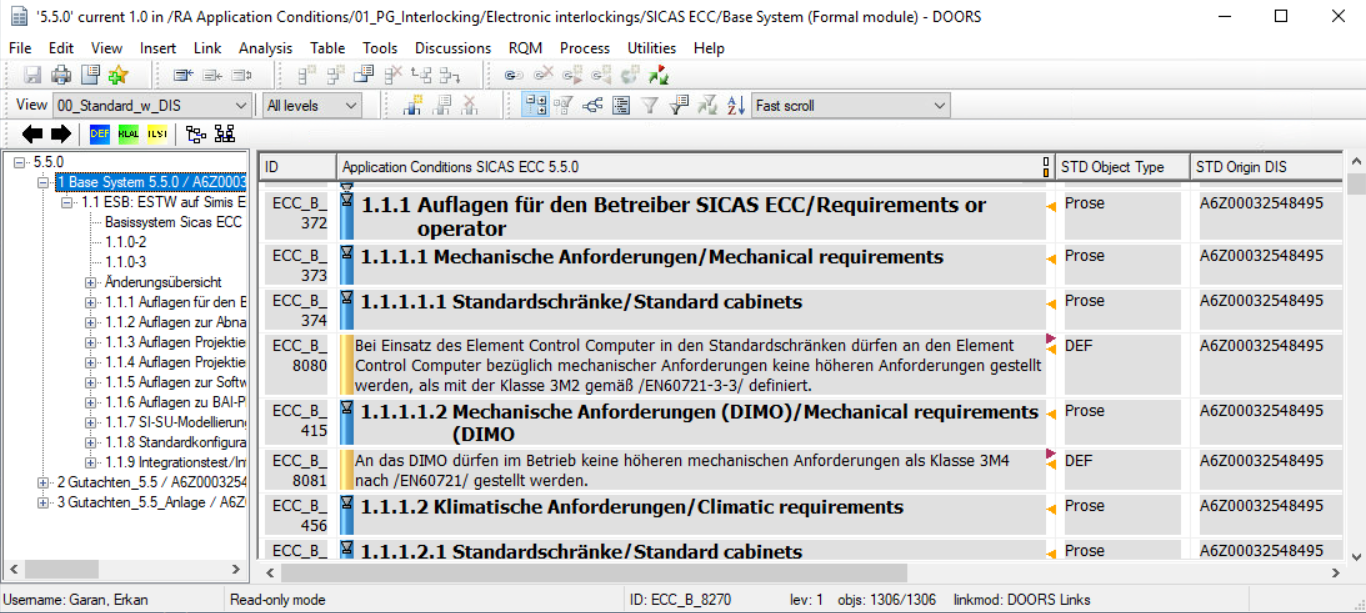
\includegraphics[width = \textwidth]{abbildungen/Modul in Doors.PNG}
    \caption{Geöffnetes Modul in \acs{DOORS}}
    \label{fig:Modul Doors}
\end{figure}

\subsection{Objekte und Attribute}
Innerhalb eines Moduls werden Daten in Objekten gespeichert. In der Regel bestehen Objekte aus mindestens zwei Spalten. Die erste 
Spalte enthält eine ID, die sich aus einem Präfix und einem Integerwert zusammensetzt. Der Integerwert wird bei jedem neu angelegtem 
Objekt inkrementiert, sodass jedem Objekt innerhalb eines Moduls eine eindeutige ID zugeordnet werden kann.
Die zweite Spalte besteht dabei entweder aus einer Sektions-Nummer und einer Überschrift, wie im ersten Objekt in der Abbildung 
\ref*{fig:Modul Doors} zu sehen ist, oder aus einem Objekt-Text, der beispielsweise eine Anforderung beinhalten kann. Ein Beispiel für 
einen Objekt-Text, der eine Anforderung beinhaltet, ist das vierte Objekt der Abbildung \ref*{fig:Modul Doors} \cite[vgl. S.178]{DOORS}.
Einem Objekt können beliebig viele weitere Attribute hinzugefügt werden. 

Attribute beinhalten relevante Informationen über Module oder Objekte. Modulattribute speichern Informationen über das Modul, wie beispielsweise
den Ersteller des Moduls, das letzte Änderungsdatum und Ähnliches. Diese Modulattribute findet der Benutzer über die Eigenschaften des Moduls, 
welche mit einem Rechtsklick auf das Modul in der grafischen Oberfläche geöffnet werden können. Objektattribute hingegen
speichern Informationen über die Objekte. In der Abbildung \ref*{fig:Modul Doors} ist die Spalte STD Object Type z.B. ein Objektattribut,
das definiert, ob es sich bei dem Objekt um eine Anforderung oder um Prosa, also z.B. eine Überschrift handelt.

\subsection{Baseline}
Eine Baseline friert den aktuellen Stand der Anforderungen eines Projekts mit ihren Attributen ein und ist eine nicht veränderbare Kopie von 
formalen Modulen \cite[vgl. S.182]{DOORS}. Baselines werden in der Regel zu Releases von Systemen oder Subsystemen erstellt \cite[vgl. S.60]{SMO-PE}. 
Wenn ein Formal Module geöffnet ist, kann der Benutzer unter File \textrightarrow{} Baseline eine Baseline erstellen oder eine bereits vorhandene 
Baseline ansehen. Abbildung \ref*{fig:Baselines} zeigt das Dialogfenster zum Öffnen bereits vorhandener Baselines. Dort wird deutlich, 
dass Baselines versioniert werden können.

\begin{figure}[H]
    \centering
    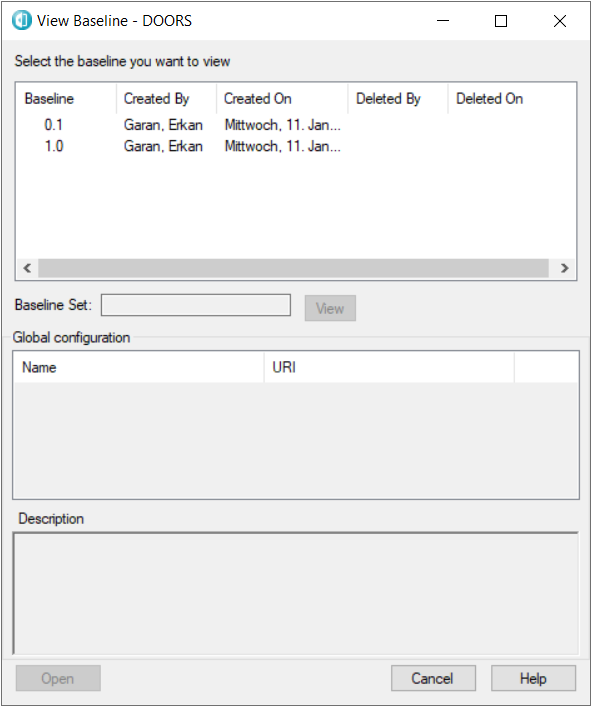
\includegraphics[scale = 0.7]{abbildungen/Baselines.PNG}
    \caption{Baselines eines Moduls in \acs{DOORS}}
    \label{fig:Baselines}
\end{figure}

\subsection{Links}
In der Abbildung \ref*{fig:Modul Doors} sind an der rechten Kante der zweiten Spalte zwei Arten von Pfeilen zu erkennen. Diese Pfeile
symbolisieren Links in \ac{DOORS}. Links sind gerichtete Verbindungen von einem Quellobjekt zu einem Zielobjekt. Sie werden in \ac{DOORS} 
genutzt, um die Verfolgbarkeit von Anforderungen zu gewährleisten. Der Benutzer kann 
dabei, ungeachtet von der Richtung des Links, vom Quellobjekt zum Zielobjekt oder andersherum navigieren \cite[vgl. S.183]{DOORS}. 
Ein nach links zeigender gelber Pfeil ist dabei ein In-Link, das heißt, dass dieses Objekt als Zielobjekt dient und ein anderes Objekt 
eine Verbindung zu diesem Objekt hat. Das Gegenstück zum In-Link ist ein Out-Link. Dieser wird in der grafischen Benutzeroberfläche von 
\ac{DOORS} als roter nach rechts zeigender Pfeil dargestellt. Hat ein Objekt einen Out-Link, heißt das, dass dieses Objekt als Quellobjekt 
dient und eine Verbindung zu einem anderen Objekt, welches als Zielobjekt dient, hat.   

\subsection{DXL}

\ac{DXL} ist eine Skript-Sprache, die ein Teil des Anforderungsmanagement-Tools \ac{DOORS} ist. Durch diese Skript-Sprache
können Skripte geschrieben werden, die als Batch-Skript ausgeführt werden können. Diese Skripte bieten neben der grafischen Benutzeroberfläche eine weitere Möglichkeit, 
um mit \ac{DOORS} zu arbeiten. Zudem besteht die Möglichkeit die grafische Benutzeroberfläche von \ac{DOORS} um neue, entwickelte Anwendungen zu
erweitern. Von der Syntax ähnelt die Sprache den Programmiersprachen C und C++ \cite[vgl. S.1]{DXL}. Eine Besonderheit von \ac{DXL} ist dabei der Datentyp Skip, 
welche eine Skiplist als Datenstruktur implementiert. Eine Skiplist besteht aus Key-Value-Paaren und ermöglicht einen schnellen Zugriff auf einzelne Elemente.

\ac{DXL} wurde im Praxisprojekt zum Sammeln von Bewertungen von Anwendungsregeln aus Projekten der Siemens Mobility GmbH 
genutzt, indem Batch-Skripte geschrieben wurden. Diese Skripte haben im zentralen Projekt, das die Anwendungsregeln von Komponenten beinhaltet, die Links der Objekte
verfolgt und dort in den Modulen nach korrekt bewerteten Anwendungsregeln gesucht. Diese wurden dann nach Projekt und Komponente gruppiert und 
jeweils in neue Module geschrieben, um in Zukunft als Lösungsvorschlag für neue Projekte zu dienen. Der Inhalt dieser Module wird als Datensatz für diese Bachelorarbeit genutzt.
Ebenfalls wird \ac{DOORS} dazu benötigt, um in der grafischen Oberfläche eines Moduls mit neu importierten Anwendungsregeln ein Programm zu starten, was mit den Informationen aus dem Modul
ein weiteres Skript in der Programmiersprache Python startet. In dem Python-Skript wird das KI-Modell erstellt und angelernt. Mithilfe des Modells und mit den Daten über die Anwendungsregeln aus 
dem Modul soll das Modell dann Vorschläge zur Bewertung der Anwendungsregeln liefern.

